%!TEX root = ../clcxsj.tex

\chapter{平面坐标系统之间的转换}

在某些工程中,由于不知道新旧两种坐标系的建立方法或参数,因此无法用换带计算的方法
进行坐标转换。如果知道某些点在两个坐标系中的坐标值,我们就可以采用一些近似的转换方
法将其它的点也转换到新坐标系中,求出其坐标值。尤其对于较低等级的大量控制点来说,
采用这些近似方法,能够快速得到转换结果。

 \section{原理和数学模型}

\subsection{原理}
这些方法的实质是根据新旧网的重合点(又称为公共点)的坐标值之差,按一定的规律修正
旧网的各点坐标值,使旧网最恰当的配合到新网内。修正时因不合观测值改正数平方和为最
小的原则,故为近似方法。

\begin{figure}[htbp]
    \centering
    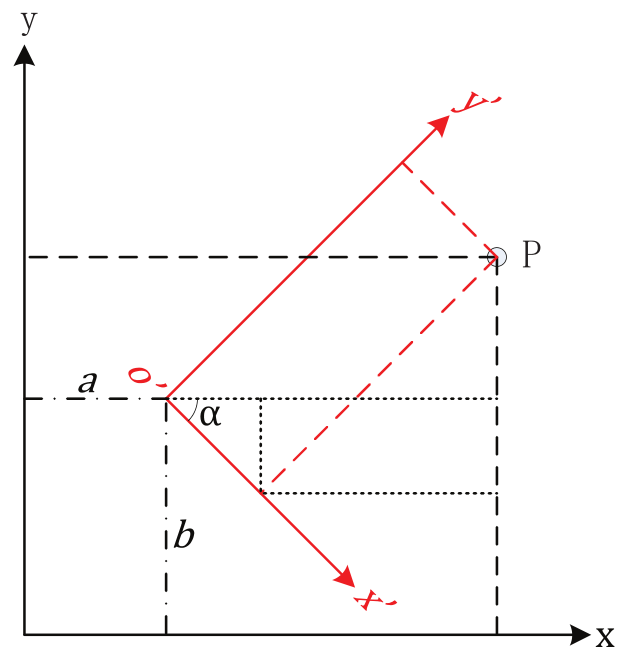
\includegraphics[scale=0.6]{xytoxy/xytoxy.png}
    \caption{坐标相似变换示意图}
    \label{fig:xytoxy}
\end{figure}

常用的方法有简单变换方法(又称赫尔默特法或相似变换法)、仿射变换法、正形变换法等。
在这里我们主要讲解简单变换法。

\subsection{相似变换法的数学模型}
实质是使旧网坐标系平移、旋转和进行尺度因子改正,将旧网配合到新网上。因旧网形状保
持不变,故称为平面相似变换法。

变换方程为:
$$\left.
\begin{array}{l}
\textrm{$x=a+k(x'\cos\alpha+y'\sin\alpha)$} \\
\textrm{$y=b+k(-x'\sin\alpha+y'\cos\alpha)$}
\end{array}\right\}$$

式中$a$,$b$表示平移,$\alpha$是旧网$x'$轴逆转至新网$x$轴的转角,$k$为尺度因子。
这些变换参数是未知的,要根据新旧网公共点上的已知坐标$x$,$y$和$x'$、$y'$求解确定。

因此必须至少有两个公共点,列出四个方程式,解算出这四个未知参数值。如果具有两个以
上的公共点时,就应该应用最小二乘平差方法,求解最或是参数值。

为解算出这些参数,我们引入参数$c$、$d$:

$c=k\cos\alpha$,$d=k\sin\alpha$

将公式转换为:
$$\left.
\begin{array}{l}
\textrm{$x=a+x'c+y'd$}\\
\textrm{$y=b+y'c-x'd¥$}
\end{array}\right\}$$

由于新旧网都存在测量误差,设新旧坐标$x$,$y$和$x'$,$y'$的误差分别为
$v_x$,$v_y$和$v_{x'}$,$v_{y'}$,因此上式改写为:

$$\left.\begin{array}{l}
\textrm{$x+v_x=a+(x'+v_{x'})c+(y'+v_{y'})d$} \\
\textrm{$y+v_y=b+(y'+v_{y'})c-(x'+v_{x'})d$}
\end{array}\right\}$$

设:
$$\left.\begin{array}{l}
\textrm{$n_x=-v_x+cv_{x'}+dv_{y'}$} \\
\textrm{$n_y=-v_y-dv_{x'}+cv_{y'}$}
\end{array}\right\}$$

则有:
$$\left.\begin{array}{l}
\textrm{$-n_x=a+x'c+y'd-x$} \\
\textrm{$-n_y=b+y'c-x'd-y$}
\end{array}\right\}$$

若有$r$个新旧网的公共点,则可组成$r$对方程:
$$V=BX-l$$

上式即为参数平差时的方程,$l$代表观测向量,$V$代表改正数向量,$B$代表系数矩阵,
$X$是参数向量。它们的值为:

$\mathbf{V}=
\left(\begin{array}{c}
-n_{x1} \\ -n_{y1} \\ \vdots \\ -n_{xr} \\ -n_{yr}
\end{array}\right)$
$\mathbf{B}=
\left(\begin{array}{cccc}
1 & 0 & x'_1 & y'_1 \\
0 & 1 & y'_1 & -x'_1 \\
\dots & \dots & \ldots & \ldots \\
1 & 0 & x'_r & y'_r \\
0 & 1 & y'_r & -x'_r
\end{array}\right)$
$\mathbf{X}=
\left(\begin{array}{c}
a \\ b \\ c \\ d
\end{array}\right)$
$\mathbf{l}=
\left(\begin{array}{c}
x_1 \\ y_1 \\ \vdots \\ x_r \\ y_r
\end{array}\right)$

根据最小二乘原理$V^TV=min$可得到法方程:
$$B^TBX-B^Tl=0$$

解法方程可求得$a$、$b$、$c$、$d$的值:
$$X=(B^TB)^{-1}(B^Tl)$$

旋转角$\alpha$和尺度比$k$为:
$$\alpha=\arctan\frac{d}{c}$$
$$k=\sqrt{c^2+d^2}$$
之后,就可计算旧网中所有待转换点的新坐标。

\section{程序功能设计}
从数学模型可看出,程序的关键是矩阵解算,其次是数据的组织问题。我们首先考虑数据文件的组织格式。

\subsection{数据文件和成果文件格式}
由于程序的功能较为单一,数据文件的格式也较为简单。我们设计格式如下:
\begin{verbatim*}
公共点个数
待转换点个数
//公共点在旧坐标系中的坐标
点名 x坐标 y坐标
................
//公共点在新坐标系中的坐标
点名 x坐标 y坐标
................
//待转换点在旧坐标系中的坐标
点名 x坐标 y坐标
................
\end{verbatim*}

我们设计成果文件的格式如下:
\begin{verbatim}
公共点个数 待转换点个数
===公共点在旧坐标系中的坐标===
点名 x坐标 y坐标
................
===公共点在新坐标系中的坐标===
点名 x坐标 y坐标
................
===待转换点在旧坐标系中的坐标===
点名 x坐标 y坐标
................
转换参数(平移量a)、(平移量b)、(旋转角α )、(尺度比k)
转换的精度
===待转换点在新坐标系中的坐标===
点名 x坐标 y坐标
................
\end{verbatim}

\subsection{程序流程}
根据以上分析,程序流程如下:
\begin{enumerate}
 \item 读取公共点旧坐标
  \item 读取公共点新坐标
  \item 组成误差方程式
  \item 解算参数向量
  \item 解算待定点的坐标
  \item 将计算成果写入文件
\end{enumerate}


\subsection{主要功能设计}
为了实现以上功能,我们需要设计一个结构(或类)用于表示点,设计如下:
\begin{verbatim}
struct Pnt
{
    char _name[11];
    double _oldx, _oldy, _newx, _newy;
};
\end{verbatim}

同时,我们设计另一个类$CoordSys$来完成相应的其它功能:
\begin{verbatim}
class CoordSys
{
private:
    double _a, _b, _alpha, _k;
    int _n0, _ni;
    Pnt * _pPnts;
public:
    CoordSys(void);
    ~CoordSys(void);

    Pnt * GetPnt(const char * name);
    void ReadPntCount(FILE * in);
    void ReadCommontPntOldXY(FILE * in);
    void ReadCommontPntNewXY(FILE * in);
    void ReadUnKnownPnt(FILE * in);

    void ReadData(FILE * in);

    void WritePntCount(FILE * out);
    void WriteCommontPntOldXY(FILE * out);
    void WriteCommontPntNewXY(FILE * out);
    void WriteUnKnownPntOldXY(FILE * out);
    void WriteUnKnownPntNewXY(FILE * out);
    void WriteABK(FILE * out);

    void WriteData(FILE * out);
    void NegativeMatrix(double A[], double B[], int n);
    void Cal();
};

CoordSys::CoordSys(void)
{
    _a = _b = _alpha = _k = 0;
    _n0 = _ni = 0;
    _pPnts = NULL;
}

CoordSys::~CoordSys(void)
{
    if(_pPnts != NULL)
    {
        delete[] _pPnts;
        _pPnts = NULL;
    }
}

void CoordSys::ReadPntCount(FILE * in)
{
    fscanf(in,"%d", &_n0); //读入公共点个数
    fscanf(in,"%d", &_ni); //读入待定点个数
    _pPnts = new Pnt[_n0 + _ni];
}

Pnt * CoordSys::GetPnt(const char * name)
{
    for(int i = 0; i<_n0; i++)
    {
        if(strcmp(_pPnts[i]._name, name) == 0)
            return &_pPnts[i];
    }
    return NULL;
}

void CoordSys::ReadCommontPntOldXY(FILE * in)
{
    char line[256];
    fscanf(in, "%s", line);
    for(int i=0; i<_n0; i++)
    {
        fscanf(in, "%s %lf %lf", _pPnts[i]._name,
             &_pPnts[i]._oldx, &_pPnts[i]._oldy);
    }
}

void CoordSys::ReadCommontPntNewXY(FILE * in)
{
    char line[256];
    fscanf(in, "%s", line);
    for(int i=0; i<_n0; i++)
    {
        char name[11];
        double x, y;

        fscanf(in, "%s %lf %lf", name, &x, &y);
        Pnt * pPnt = GetPnt(name);//此处未加容错处理
        pPnt->_newx = x;
        pPnt->_newy = y;
    }
}

void CoordSys::ReadUnKnownPnt(FILE * in)
{
    char line[256];
    fscanf(in, "%s", line);
    for(int i=0; i<_ni; i++)
    {
        fscanf(in, "%s %lf %lf", _pPnts[i+_n0]._name,
        &_pPnts[i+_n0]._oldx, &_pPnts[i+_n0]._oldy);
    }
}

void CoordSys::WritePntCount(FILE * out)
{
    fprintf(out, "公共点个数:%d\n", _n0);
    fprintf(out, "待定转换点个数:%d\n", _ni);
}
void CoordSys::WriteCommontPntOldXY(FILE * out)
{
    fprintf(out, "===公共点在旧坐标系中的坐标===\n");
    for(int i=0; i<_n0; i++)
        fprintf(out, "%s\t%lf\t%lf\n", _pPnts[i]._name,
                     _pPnts[i]._oldx, _pPnts[i]._oldy);
}
void CoordSys::WriteCommontPntNewXY(FILE * out)
{
    fprintf(out, "===公共点在新坐标系中的坐标===\n");
    for(int i=0; i<_n0; i++)
        fprintf(out, "%s\t%lf\t%lf\n", _pPnts[i]._name,
                     _pPnts[i]._newx, _pPnts[i]._newy);
}
void CoordSys::WriteUnKnownPntOldXY(FILE * out)
{
    fprintf(out, "===待转换点在旧坐标系中的坐标===\n");
    for(int i=0; i<_ni; i++)
        fprintf(out, "%s\t%lf\t%lf\n", _pPnts[i+_n0]._name,
                 _pPnts[i+_n0]._oldx, _pPnts[i+_n0]._oldy);
}
void CoordSys::WriteUnKnownPntNewXY(FILE * out)
{
    fprintf(out, "===待转换点在新坐标系中的坐标===\n");
    for(int i=0; i<_ni; i++)
        fprintf(out, "%s\t%lf\t%lf\n", _pPnts[i+_n0]._name,
                 _pPnts[i+_n0]._newx, _pPnts[i+_n0]._newy);

}
void CoordSys::WriteABK(FILE * out)
{
    fprintf(out, "转换参数:a=%lf, b=%lf, α=%lf, k=%lf\n",
                            _a,    _b, _alpha,      _k);
}

void CoordSys::ReadData(FILE * in)
{
    ReadPntCount(in);
    ReadCommontPntOldXY(in);
    ReadCommontPntNewXY(in);
    ReadUnKnownPnt(in);
}

void CoordSys::WriteData(FILE * out)
{
    WritePntCount(out);
    WriteCommontPntOldXY(out);
    WriteCommontPntNewXY(out);
    WriteUnKnownPntOldXY(out);
    WriteABK(out);
    WriteUnKnownPntNewXY(out);
}

//解法方程AX = B, A:n×n B:n×1
void CoordSys::NegativeMatrix(double A[], double B[], int n)
{
    for(int k = 0; k < n-1; k++)
    {
        for(int i = k+1; i < n; i++)
        {
            A[i*n + k] /= A[k*n + k];
            for(int j = k+1; j < n; j++)
            {
                A[i*n + j] -= A[i*n + k] * A[k*n + j];
            }
            B[i] -= A[i*n + k] * B[k];
        }
    }

    B[n-1] /= A[(n-1)*n + (n-1)];
    for(int i= n-2; i >= 0; i--)
    {
        double s = 0.0;
        for(int j = i+1; j < n; j++)
        {
            s += A[i*n + j] * B[j];
        }
        B[i] = (B[i]-s) / A[i*n + i];
    }
}
void CoordSys::Cal()
{
    double * B = new double[2*_n0 * 4];
    double * l = new double[2*_n0];
    double * N = new double[4*4];
    double * U = new double[4];

    for(int i=0; i<_n0; i++)
    {
        B[(2*i)* 4 + 0] = 1.0;
        B[(2*i)* 4 + 1] = 0.0;
        B[(2*i)* 4 + 2] = _pPnts[i]._oldx;
        B[(2*i)* 4 + 3] = _pPnts[i]._oldy;
        l[2*i] = _pPnts[i]._newx;

        B[(2*i +1)* 4 + 0] = 0.0;
        B[(2*i +1)* 4 + 1] = 1.0;
        B[(2*i +1)* 4 + 2] = _pPnts[i]._oldy;
        B[(2*i +1)* 4 + 3] = -_pPnts[i]._oldx;
        l[2*i +1] = _pPnts[i]._newy;
    }

    for(int k=0; k<4; k++)
    {
        for(int j=0; j<4; j++)
        {
            N[k*4+j] = 0.0;
            for(int i=0; i<2*_n0; i++)
            {
                N[k * 4 + j] += B[i*4 + k] * B[i*4 + j];
            }
        }

        U[k] = 0.0;
        for(int i=0; i<2*_n0; i++)
            U[k] += B[i*4 + k] * l[i];
    }
    NegativeMatrix(N, U, 4);

    _a = U[0];
    _b = U[1];
    _alpha = RadToDms(atan2(U[3], U[2]));
    _k= sqrt(U[3]*U[3]+U[2]*U[2]);

    for(int i=0; i<_ni; i++)
    {
        _pPnts[_n0+i]._newx = U[0] + U[2]* _pPnts[_n0+i]._oldx
                                   + U[3]*_pPnts[_n0+i]._oldy;
        _pPnts[_n0+i]._newy = U[1] + U[2]* _pPnts[_n0+i]._oldy
                                   - U[3]*_pPnts[_n0+i]._oldx;
   }
   delete[] N;
   delete[] l;
   delete[] B;
}

void main()
{
    CoordSys coordSys;
    FILE * in, * out;

    in = fopen("xytoxy.txt", "r"); //打开已知文件
    coordSys.ReadData(in);
    fclose(in);

    coordSys.Cal();

    out = fopen("toxy.txt", "w");
    coordSys.WriteData(out);
    fclose(out);
}
\end{verbatim}

计算示例数据文件内容:
\begin{verbatim}
3
6
//公共点在旧坐标系中的坐标
103 3927002.191 449256.848
100 3928471.180 451589.920
102 3928308.824 446388.500
//公共点在新坐标系中的坐标
103 327156.644 485664.463
100 328638.283 487989.669
102 328447.816 482788.977
//待转换点在旧坐标系中的坐标
11 3927202.638 448247.421
07 3928890.412 449425.214
15 3927466.357 446917.643
103 3927002.191 449256.848
100 3928471.180 451589.920
102 3928308.824 446388.500
\end{verbatim}

计算成果文件内容:
\begin{verbatim}
公共点个数:3
待定转换点个数:6
===公共点在旧坐标系中的坐标===
103	3927002.191000	449256.848000
100	3928471.180000	451589.920000
102	3928308.824000	446388.500000
===公共点在新坐标系中的坐标===
103	327156.644000	485664.463000
100	328638.283000	487989.669000
102	328447.816000	482788.977000
===待转换点在旧坐标系中的坐标===
11	3927202.638000	448247.421000
07	3928890.412000	449425.214000
15	3927466.357000	446917.643000
103	3927002.191000	449256.848000
100	3928471.180000	451589.920000
102	3928308.824000	446388.500000
转换参数:a=-3602385.714666, b=57613.407531,
 α =0.183446, k=1.000043
===待转换点在新坐标系中的坐标===
11	327351.643066	484653.926898
07	329045.829449	485822.634190
15	327608.184475	483322.685785
103	327156.644527	485664.465940
100	328638.281925	487989.667546
102	328447.816548	482788.975515
\end{verbatim}
